\documentclass[
    paper=a4,
    DIV14,
    fontsize=12pt,
    pagesize=pdftex,
    toc=bibliographynumbered
]{scrartcl}
\usepackage[utf8]{inputenc}
\usepackage[T1]{fontenc}
\usepackage[ngerman]{babel}
\usepackage[autostyle=true]{csquotes}
\usepackage{enumitem}
\usepackage{mathtools, amsfonts, amssymb, amsthm}
\usepackage{lmodern}
\usepackage{dsfont}

\usepackage[%
    font=footnotesize,
    margin=0.2em,
    labelfont=bf,
    format=plain,
    labelsep=endash
]{caption}
\usepackage[%
    font=footnotesize,
    margin=0.2em,
    labelfont=bf,
    format=plain,
    labelsep=endash
]{subcaption}

% stelle Fonts auf Serif
\setkomafont{sectioning}{\rmfamily\bfseries\boldmath}
\setkomafont{descriptionlabel}{\rmfamily\bfseries}
\numberwithin{figure}{section}
\numberwithin{equation}{section}
\numberwithin{table}{section}

% Mengen
\newcommand*\setZ{\mathds{Z}}
\newcommand*\setR{\mathds{R}}
\newcommand*\setN{\mathds{N}}
\newcommand*\setK{\mathds{K}}

% nummeriere besimmte Gleichung
\newcommand\numberthis{\addtocounter{equation}{1}\tag{\theequation}}

% Matrizen, Vektoren
\newcommand*\vecz[2]{\begin{pmatrix} #1 \\ #2 \end{pmatrix}}
\newcommand*\vecd[3]{\begin{pmatrix} #1 \\ #2 \\ #3 \end{pmatrix}}
\newcommand*\vecf[4]{\begin{pmatrix} #1 \\ #2 \\ #3 \\ #4 \end{pmatrix}}
\newcommand*\matDD[4]{\begin{pmatrix} #1 & #2 \\ #3 & #4 \end{pmatrix}}
\newcommand*\diff{\mathrm d}

\title{Immer der Sonn' entgegen}
\subtitle{Proseminar: Mathematische Modellierung}
\author{Dominik Bendle, Melissa Hasel, Thomas Hofmann}
\date{Wintersemester 2016/17}

\begin{document}
\begin{titlepage}
    \maketitle
    \thispagestyle{empty}
    \centering
    \vfill
    % hier passendes Bild einfügen
    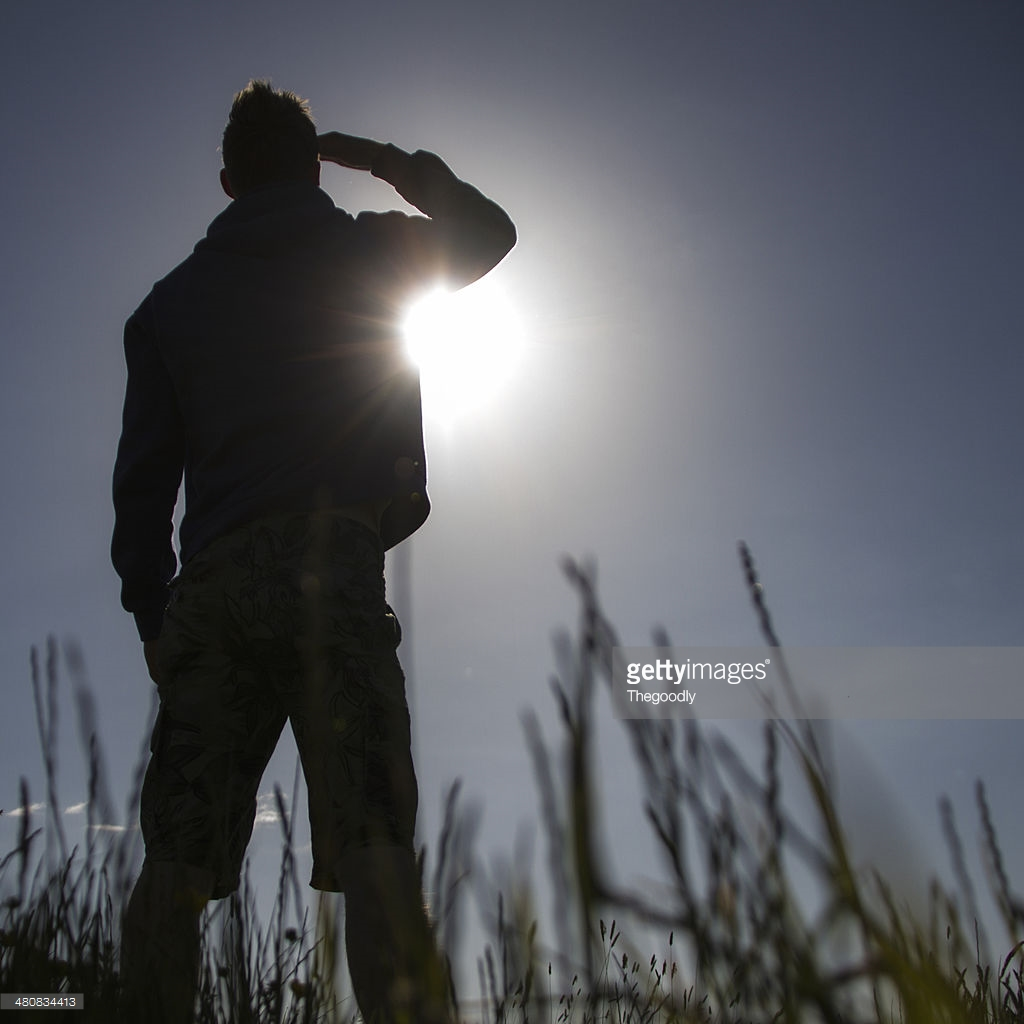
\includegraphics[width=0.6\textwidth]{images/man_looking_at_sun.jpg}
    \vfill
\end{titlepage}

\tableofcontents
\vfill
\listoffigures
\newpage
\pagestyle{headings}

\section{Problembeschreibung}
Wir beschäftigen uns mit der in folgender Erzählung aufkommender Problemstellung:
\blockquote{
    Peter rüttelte herrscherlich sein Gabelzepter über die Flämmchen, die sogleich gefällig
    zischelnd höher wucherten; stieß die Zinken in den Boden; drapierte die verschränkten
    Arme dicker auf den Stiel, und erkundigte sich tiefsinnig:

    \textit{Wo käm' man da eigentlich hin? Wenn man immerfort \enquote{Der Sonn' entgegen}
    ginge?}

    \textit{Von morgens an? Na, da würd's'De abends wieder am Ausgangspunkt sein},
    entschied ich, voreilig wie immer \dots

    \textit{Nein. Neinein}, sagte er: \textit{Davon kann gar keine Rede sein, daß man
    abends wieder am Ausgangspunkt wäre. Das ist sogar eine ziemlich komplizierte
    Angelegenheit. Zuerst ginge man nach Osten. Dann nach Süden ausholen. Dann, im Laufe
    des Nachmittags, Süd-West…und schließlich nach Westen: immer der Sonn' entgegen.}

    \textit{Am einfachsten wäre's, man führte das Experiment einmal praktisch durch.}

    \textit{Wie, zum Beispiel, der Sonn' entgegen zu gehen. Ich sag' Dir bloß das Eine:
    wenn ich unterwegs an einem Strunk eine KIEFERNGLUCKE erblicken sollte: die wird
    geerntet!}

    \textit{Kannst Du Dir nicht Sparassis ramosa merken, Peter?} tadelte Fritz:
    \textit{Eine Unterbrechung kommt selbstverständlich überhaupt nicht infrage. Und wenn
    uns ein ganzer Harem verlockend in den Weg tänzelte!}
}

Konkret wollen wir also bei gegebenem Startpunkt und -datum bestimmen, welche Route
entsteht, wenn wir von Sonnenauf- bis Sonnenuntergang immer der Sonne  hinterherlaufen
oder -wandern.

\section{Übersicht}

\end{document}
